%&./out/hands-on-ml_slides_chapter-10-1st-half
% use precompiled file
%%%%%%%%%% ↑ EDIT FILE NAME ↑ %%%%%%%%%%

% @file           hands-on-ml_slides_chapter-10-1st-half.tex
% @author         Kataoka Nagi
% @date           2021-04-08 04:48:00
% $Version:       1.0
% @par            History
%                 New file
% Copyright (c) 2021 Kataoka Nagi
% - This src is released under the MIT License, see LICENSE.
%
% \documentclass[dvipdfmx, 11pt]{beamer}^
% aspectratio = 43, 149, 169
% font size = 8pt, 9pt, 10pt, 11pt, 12pt, 14pt, 17pt, 20pt
% @see 「Beamer columns 環境で画像を配置するベストな方法」https://qiita.com/t_uda/items/8ef173eebf9827305135#3-columns-%E7%92%B0%E5%A2%83%E3%81%AE%E6%AD%A3%E3%81%97%E3%81%84%E4%BD%BF%E3%81%84%E6%96%B9
\PassOptionsToClass{hiresbb}{graphicx}
\documentclass[aspectratio=169, dvipdfmx, 14pt, xcolor={svgnames,dvipsnames}]{beamer}
\usepackage{graphicx}
\newcommand{\thickhrulefill}{\leavevmode\leaders\hrule depth-1.2pt height 3.2pt\hfill\kern0pt}
\newcommand{\indicatewidth}[1]{\thickhrulefill{#1}\thickhrulefill}
\newlength{\mytotalwidth}
\mytotalwidth=\dimexpr\linewidth-5mm
\newlength{\mycolumnwidth}
\mycolumnwidth=\dimexpr\mytotalwidth-5mm

\usepackage{base_kataoka-nagi}
\usepackage{slides_kataoka-nagi}
% \usepackage{../styles/base_kataoka-nagi/base_kataoka-nagi} % debug
% \usepackage{../styles/slides_kataoka-nagi/slides_kataoka-nagi} % debug

% precompile preamble from here. don't precompile with glossaries-env!
% type [eptex -ini -jobname="FILE_NAME" "&platex" mylatexformat.ltx FILE_NAME.tex] in cd
% @see 「beamerのコンパイル速度を上げる」 http://margaret-sdpara.blogspot.com/2019/11/beamer.html
\endofdump

\def\tightlist{\itemsep1pt\parskip0pt\parsep0pt}
% \includeonlyframes{current} % current build \begin{frame}[\quad label=current]

% \usepackage{enumitem}
% \setlistdepth{10}
% \renewlist{itemize}{itemize}{10}
\setbeamertemplate{itemize subsubitem}{\tiny\raise2pt\hbox{■}}

\title[実践機械学習 輪読会 第10章 前半]{scikit-learn、Keras、TensorFlowによる\\実践機械学習 第2版\\第10章 前半}
\subtitle{データ工学研究室 輪読会}
\author[片岡 凪]{AL18036 片岡 凪}
% \institute[SIT]{芝浦工業大学 工学部 情報工学科 4年}
\institute[データ工学研究室 B4]{芝浦工業大学 工学部 情報工学科 4年}
\date{Apr. 8th, 2021}

\begin{document}

%%%%%%%%%%%%%%%%%%%%%%%%%%%%%%%%%%%%%%%%%%%%%%%%%%

\maketitle

%%%%%%%%%%%%%%%%%%%%%%%%%%%%%%%%%%%%%%%%%%%%%%%%%%

% \begin{frame}[\quad label=current]{\quad 発表者}
\begin{frame}{\quad 発表者紹介}
  \begin{columns}[totalwidth=\mytotalwidth]
    \begin{column}[t]{0.8\mycolumnwidth}
      \begin{itemize}
        \item 片岡 凪
        \item 千葉県 浦安市
        \item 芝浦工業大学 工学部 情報工学科 4年
        \item データ工学研究室(木村昌臣研究室)
        \item 関心:画像,XAI,自動化,効率化
        \item Twitter @calm\_IRL
        \item Github  KataokaNagi
      \end{itemize}
    \end{column}
    \begin{column}[T]{0.2\mycolumnwidth}
      \centering
      
\includegraphics[width=80pt]{img/icon.jpg}
    \end{column}
  \end{columns}
\end{frame}

%%%%%%%%%%%%%%%%%%%%%%%%%%%%%%%%%%%%%%%%%%%%%%%%%%

% index
\begin{frame}{\quad 目次}
  \tableofcontents
\end{frame}

% \begin{frame}{\quad ブロック環境}
%   \begin{block}{block}
%     block
%   \end{block}
%   \begin{alertblock}{alertblock}
%     alertblock
%   \end{alertblock}
%   \begin{exampleblock}{exampleblock}
%     exampleblock
%   \end{exampleblock}
%   \begin{tcolorbox}[colframe=green,
%       colback=green!10!white,
%       colbacktitle=green!40!white,
%       coltitle=black, fonttitle=\bfseries,
%       title=My box]
%     box contents
%   \end{tcolorbox}
% \end{frame}

%%%%%%%%%%%%%%%%%%%%%%%%%%%%%%%%%%%%%%%%%%%%%%%%%%

\section{第10章 人工ニューラルネットワークとKerasの初歩}
\begin{frame}{\quad 目次}
  \tableofcontents[currentsection]
\end{frame}

%%%%%%%%%%%%%%%%%%%%%%%%%%%%%%%%%%%%%%%%%%%%%%%%%%

\begin{frame}{\quad 第10章 概要}
  \begin{itemize}
    \tightlist
    \item
          ANN(Artifical NN)
    \item
          MLP(Multi-layer Perceptron)
    \item
          Keras API
    \item
          ※ ユニット = ニューロン

          \begin{itemize}
            \tightlist
            \item
                  生物学的な意味に制限しないための用語
          \end{itemize}
  \end{itemize}

\end{frame}

%%%%%%%%%%%%%%%%%%%%%%%%%%%%%%%%%%%%%%%%%%%%%%%%%%

\hypertarget{ux751fux7269ux5b66ux7684ux306aux30cbux30e5ux30fcux30edux30f3ux304bux3089ux4ebaux5de5ux30cbux30e5ux30fcux30edux30f3ux3078}{%
  \section{10.1
    生物学的なニューロンから人工ニューロンへ}\label{ux751fux7269ux5b66ux7684ux306aux30cbux30e5ux30fcux30edux30f3ux304bux3089ux4ebaux5de5ux30cbux30e5ux30fcux30edux30f3ux3078}}
\begin{frame}{\quad 目次}
  \tableofcontents[currentsection]
\end{frame}

%%%%%%%%%%%%%%%%%%%%%%%%%%%%%%%%%%%%%%%%%%%%%%%%%%

\begin{frame}{\quad ANNの歴史1}
  \begin{itemize}
    \tightlist
    \item
          1943

          \begin{itemize}
            \tightlist
            \item
                  ANN
            \item
                  命題論理
          \end{itemize}
    \item
          1960s

          \begin{itemize}
            \tightlist
            \item
                  コネクショニズム(NNの研究)
          \end{itemize}
    \item
          1990

          \begin{itemize}
            \tightlist
            \item
                  SVM
          \end{itemize}
  \end{itemize}
\end{frame}

%%%%%%%%%%%%%%%%%%%%%%%%%%%%%%%%%%%%%%%%%%%%%%%%%%

\begin{frame}{\quad ANNの歴史2}
  \begin{itemize}
    \item
          近年

          \begin{itemize}
            \tightlist
            \item
                  \alert{ANN再燃?}

                  \begin{itemize}
                    \tightlist
                    \item
                          膨大なデータ
                    \item
                          ムーアの法則
                    \item
                          アルゴリズムの改良
                    \item
                          局所的な最適値は意外と無害
                    \item
                          流行りと資金
                  \end{itemize}
          \end{itemize}
  \end{itemize}
\end{frame}

%%%%%%%%%%%%%%%%%%%%%%%%%%%%%%%%%%%%%%%%%%%%%%%%%%

\hypertarget{ux751fux7269ux5b66ux7684ux30cbux30e5ux30fcux30edux30f3}{%
  \subsection{10.1.1
    生物学的ニューロン}\label{ux751fux7269ux5b66ux7684ux30cbux30e5ux30fcux30edux30f3}}
\begin{frame}{\quad 目次}
  \tableofcontents[currentsubsection]
\end{frame}

%%%%%%%%%%%%%%%%%%%%%%%%%%%%%%%%%%%%%%%%%%%%%%%%%%

\begin{frame}{\quad BNNの構造}
  \begin{itemize}
    \item
          細胞体
    \item
          樹状突起
    \item
          軸索

          \begin{itemize}
            \tightlist
            \item
                  細胞体の数倍から数万倍の長さ
          \end{itemize}
    \item
          終末分岐
    \item
          シナプス終端
  \end{itemize}
\end{frame}

%%%%%%%%%%%%%%%%%%%%%%%%%%%%%%%%%%%%%%%%%%%%%%%%%%

\begin{frame}{\quad BNNの挙動}
  \begin{itemize}
    \item
          活動電位(AP)か信号
    \item
          シナプスからの神経伝達物質
    \item
          発火
  \end{itemize}
\end{frame}

%%%%%%%%%%%%%%%%%%%%%%%%%%%%%%%%%%%%%%%%%%%%%%%%%%

\hypertarget{ux30cbux30e5ux30fcux30edux30f3ux306bux3088ux308bux8ad6ux7406ux6f14ux7b97}{%
  \subsection{10.1.2
    ニューロンによる論理演算}\label{ux30cbux30e5ux30fcux30edux30f3ux306bux3088ux308bux8ad6ux7406ux6f14ux7b97}}
\begin{frame}{\quad 目次}
  \tableofcontents[currentsubsection]
\end{frame}

%%%%%%%%%%%%%%%%%%%%%%%%%%%%%%%%%%%%%%%%%%%%%%%%%%

\begin{frame}{\quad ニューロン}
  \begin{itemize}
    \tightlist
    \item
          複数のバイナリ入力

          \begin{itemize}
            \tightlist
            \item
                  2つ以上の1が入力されると1となる
          \end{itemize}
    \item
          1つのバイナリ出力

          \begin{itemize}
            \tightlist
            \item
                  分岐も可能だが両方同じ値
          \end{itemize}
    \item
          \alert{任意の論理命題に対応}

          \begin{itemize}
            \tightlist
            \item
                  恒等写像
            \item
                  AND
            \item
                  OR
            \item
                  NOT(以下を組み合わせる)

                  \begin{itemize}
                    \tightlist
                    \item
                          1によって出力を禁止する機構
                    \item
                          常に1であるニューロン
                  \end{itemize}
          \end{itemize}
  \end{itemize}
\end{frame}

%%%%%%%%%%%%%%%%%%%%%%%%%%%%%%%%%%%%%%%%%%%%%%%%%%

\hypertarget{ux30d1ux30fcux30bbux30d7ux30c8ux30edux30f3}{%
  \subsection{10.1.3
    パーセプトロン}\label{ux30d1ux30fcux30bbux30d7ux30c8ux30edux30f3}}
\begin{frame}{\quad 目次}
  \tableofcontents[currentsubsection]
\end{frame}

%%%%%%%%%%%%%%%%%%%%%%%%%%%%%%%%%%%%%%%%%%%%%%%%%%

\begin{frame}{\quad パーセプトロン}
  \begin{itemize}
    \item
          ANNアーキテクチャ
    \item
          TLU(Threshold Logic Unit:閾値論理素子)のNW

          \begin{itemize}
            \tightlist
            \item
                  別名 LTU(Linear Threshold Unit:線形閾値素子)
            \item
                  人工ニューロン
            \item
                  入力の加重総和 $\bm{x}^T \bm{w}$ をステップ関数(後述)に代入
            \item
                  単体でもNNのように機能
          \end{itemize}
    \item
          接続重み
  \end{itemize}
\end{frame}

%%%%%%%%%%%%%%%%%%%%%%%%%%%%%%%%%%%%%%%%%%%%%%%%%%

\begin{frame}{\quad ステップ関数}
  \begin{itemize}
    \item
          ヘヴィサイドステップ関数

          \begin{itemize}
            \tightlist
            \item
                  heaviside(z)
            \item
                  0以上で1
          \end{itemize}
    \item
          符号関数

          \begin{itemize}
            \tightlist
            \item
                  sgn(z)
            \item
                  0は0
            \item
                  他は符号付きの1
          \end{itemize}
  \end{itemize}
\end{frame}

%%%%%%%%%%%%%%%%%%%%%%%%%%%%%%%%%%%%%%%%%%%%%%%%%%

\begin{frame}{\quad 全結合層(密層)}
  \begin{itemize}
    \item
          \alert{前の層の全てのニューロンが次の全てのニューロンに接続}
    \item
          パーセプトロンも全結合層

          \begin{itemize}
            \tightlist
            \item
                  入力層には恒等写像の入力ニューロン
            \item
                  1を出力するバイアスニューロン
          \end{itemize}
    \item
          出力 $h\_\{\bm{w}, \bm{b}\} (\bm{x}) = \phi(\bm{x}\bm{w} + \bm{b})$

          \begin{itemize}
            \tightlist
            \item
                  $\bm{x}$:インスタンスごとに1行、特徴量ごとに1列
            \item
                  $\bm{w}$:入力ニューロンごとに1行、直近の層のニューロンあたりに1列
            \item
                  $\bm{b}$:バイアスベクトル
            \item
                  $\phi$:ステップ関数などの活性化関数
          \end{itemize}
  \end{itemize}
\end{frame}

%%%%%%%%%%%%%%%%%%%%%%%%%%%%%%%%%%%%%%%%%%%%%%%%%%

\begin{frame}{\quad パーセプトロンの訓練}
  \begin{itemize}
    \item
          ヘッブの法則(ヘッブ学習)

          \begin{itemize}
            \tightlist
            \item
                  同時に発火するニューロン同士の重みを強化
          \end{itemize}
    \item
          誤った予測をしたニューロンの重みを上げる

          \begin{itemize}
            \tightlist
            \item
                  $w_{i,j}^{(next\ step)} = w_{i,j} + \eta(y_j - \hat{y}_j)x_i$
          \end{itemize}
    \item
          パーセプトロンの収束定理

          \begin{itemize}
            \tightlist
            \item
                  層の境界が線形なので複雑なパターンには向かないが,\\
                  訓練インスタンスが\alert{線形分離可能なら解が収束}
          \end{itemize}
  \end{itemize}
\end{frame}

%%%%%%%%%%%%%%%%%%%%%%%%%%%%%%%%%%%%%%%%%%%%%%%%%%

\begin{frame}{\quad 単一TLUのパーセプトロンの実装}
  \begin{itemize}
    \tightlist
    \item
          scikit-learnのPerceptionクラス
    \item
          確率的勾配降下法の特別なケースと等価
    \item
          ハード投票分類をするだけ

          \begin{itemize}
            \tightlist
            \item
                  排他的ORのような簡単な問題も解けない
            \item
                  確率を出力するロジスティック回帰の方が優れている
            \item
                  MLP(Multi-layer Perceptron:多層パーセプトロン)で解決
          \end{itemize}
  \end{itemize}
  \begin{figure}[H]
    \centering
    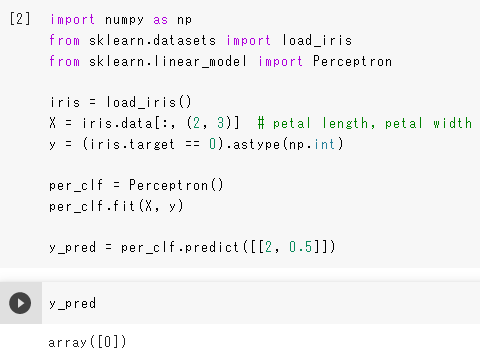
\includegraphics[width=50mm]{img/perceptron_iris.png}
    %  \caption{【キャプション名】}
    %  \label{【ラベル名】}
  \end{figure}
  % \noindent
\end{frame}

%%%%%%%%%%%%%%%%%%%%%%%%%%%%%%%%%%%%%%%%%%%%%%%%%%

\begin{frame}{\quad MLPのXOR}
  \begin{itemize}
    \item
          図で確認
  \end{itemize}
\end{frame}

%%%%%%%%%%%%%%%%%%%%%%%%%%%%%%%%%%%%%%%%%%%%%%%%%%

\hypertarget{mlpux3068ux30d0ux30c3ux30afux30d7ux30edux30d0ux30b1ux30fcux30b7ux30e7ux30f3}{%
  \subsection{10.1.4
    MLPとバックプロバケーション}\label{mlpux3068ux30d0ux30c3ux30afux30d7ux30edux30d0ux30b1ux30fcux30b7ux30e7ux30f3}}
\begin{frame}{\quad 目次}
  \tableofcontents[currentsubsection]
\end{frame}

%%%%%%%%%%%%%%%%%%%%%%%%%%%%%%%%%%%%%%%%%%%%%%%%%%

\begin{frame}{\quad MLP}
  \begin{itemize}
    \tightlist
    \item
          入力層、複数のTLU層、出力層
    \item
          出力層に近いほど上位層、遠いほど下位層と呼ばれる

          \begin{itemize}
            \tightlist
            \item
                  一方通行なアーキテクチャをFNN(Feedforward NN:順伝搬型NN)
          \end{itemize}
    \item
          出力層以外にバイアスニューロン

          \begin{itemize}
            \tightlist
            \item
                  通常は省略される
          \end{itemize}
  \end{itemize}
\end{frame}

%%%%%%%%%%%%%%%%%%%%%%%%%%%%%%%%%%%%%%%%%%%%%%%%%%

\begin{frame}{\quad DNN}
  \begin{itemize}
    \item
          ANNが深い隠れ層をもったもの

          \begin{itemize}
            \tightlist
            \item
                  層の数は曖昧になってきている
          \end{itemize}
    \item
          深層学習という分野で研究されるもの
    \item
          1986 \alert{バックプロバケーション(誤差逆伝播法)}で再燃

          \begin{itemize}
            \tightlist
            \item
                  勾配降下法の自動化(リバースモードの自動微分)

                  \begin{itemize}
                    \tightlist
                    \item
                          高速
                    \item
                          正確
                    \item
                          微分対象が様々な変数を持ち、出力が少ない場合に最適
                  \end{itemize}
            \item
                  往復1回で重みの誤差の勾配がわかる
          \end{itemize}
  \end{itemize}
\end{frame}

%%%%%%%%%%%%%%%%%%%%%%%%%%%%%%%%%%%%%%%%%%%%%%%%%%

\begin{frame}{\quad バックプロバケーション}
  \begin{itemize}
    \item
          1度に1個の\alert{ミニバッチ}(複数インスタンス)を処理(\alert{1エポック})
    \item
          手順

          \begin{itemize}
            \tightlist
            \item
                  全ての接続重みを無作為に初期化

                  \begin{itemize}
                    \tightlist
                    \item
                          対称性のある初期化をすると、ニューロンが少ないNNのように表現力が下がる
                  \end{itemize}
            \item
                  前進パス

                  \begin{itemize}
                    \tightlist
                    \item
                          処理結果を記録しつつ下位層から順に処理
                  \end{itemize}
            \item
                  後退パス

                  \begin{itemize}
                    \tightlist
                    \item
                          出力誤差をコスト関数で評価
                    \item
                          連鎖律で個々の出力接続部の誤差を計算
                  \end{itemize}
            \item
                  勾配降下ステップ

                  \begin{itemize}
                    \tightlist
                    \item
                          誤差が小さくなるように接続重みを調節
                  \end{itemize}
          \end{itemize}
  \end{itemize}
\end{frame}

%%%%%%%%%%%%%%%%%%%%%%%%%%%%%%%%%%%%%%%%%%%%%%%%%%

\begin{frame}{\quad バックプロバケーションのための改良}
  \begin{itemize}
    \item
          活性化関数の改良

          \begin{itemize}
            \tightlist
            \item
                  ステップ関数\alert{(カクカク)} -\textgreater{}
                  ロジスティック関数\alert{(滑らか)}

                  \begin{itemize}
                    \tightlist
                    \item
                          \alert{連鎖律のために勾配が取れるように}
                    \item
                          生物学的ニューロンに近しい
                  \end{itemize}
            \item
                  双曲線正接

                  \begin{itemize}
                    \tightlist
                    \item
                          $tanh(z) = 2\sigma(2z)-1$
                    \item
                          $-1 < tanh(z) < 1$
                          のため、出力が0を中心として散らばり収束が早まる
                  \end{itemize}
            \item
                  ReLU関数

                  \begin{itemize}
                    \tightlist
                    \item
                          $ReLU(z) = max(0, z)$
                    \item
                          勾配が $z = 0$ で発散し、$z < 0$
                          で$0$となるが、高速で\alert{最も利用される}
                    \item
                          出力の最大値がないため、\alert{勾配消失問題を解決する}(11章で詳解)
                  \end{itemize}
            \item
                  そもそも活性化関数は、線形関数の組み合わせで\\線形問題しか解けなかった問題を解消するための非線形関数
          \end{itemize}
  \end{itemize}
\end{frame}

%%%%%%%%%%%%%%%%%%%%%%%%%%%%%%%%%%%%%%%%%%%%%%%%%%

\hypertarget{ux56deux5e30mlp}{%
  \subsection{10.1.5 回帰MLP}\label{ux56deux5e30mlp}}
\begin{frame}{\quad 目次}
  \tableofcontents[currentsubsection]
\end{frame}

%%%%%%%%%%%%%%%%%%%%%%%%%%%%%%%%%%%%%%%%%%%%%%%%%%

\begin{frame}{\quad MLPによる回帰タスク}
  \begin{itemize}
    \item
          予測の数 = 出力ニューロンの数
    \item
          出力ニューロンには活性化関数は用いないことが多い

          \begin{itemize}
            \tightlist
            \item
                  回帰では任意の値を出力させるため
          \end{itemize}
    \item
          正の数に限定するのであれば\\ReLU関数やsoftplus関数を用いることも

          \begin{itemize}
            \tightlist
            \item
                  $softplus(z) = ln(1 + exp(z))$
          \end{itemize}
    \item
          予測値の範囲を制限するには\\ロジスティック関数や双極正接関数に通してスケーリング
  \end{itemize}
\end{frame}

%%%%%%%%%%%%%%%%%%%%%%%%%%%%%%%%%%%%%%%%%%%%%%%%%%

\begin{frame}{\quad 回帰MLPのコスト関数}
  \begin{itemize}
    \item
          平均二乗誤差 $\displaystyle \frac{1}{n}\sum_{i=1}^n(y_i-\bar{y})^2$

          \begin{itemize}
            \tightlist
            \item
                  デファクトスタンダード
          \end{itemize}
    \item
          平均絶対誤差 $\displaystyle \frac{1}{n}\sum_{i=1}^n|y_i-\bar{y}|$

          \begin{itemize}
            \tightlist
            \item
                  2乗しないので外れ値に強い
          \end{itemize}
    \item
          フーバー損失関数 $L_\delta(y, f(x))$

          \begin{itemize}
            \tightlist
            \item
                  誤差が閾値(一般に1)以下のとき \qquad $|y - f(x)| \leq \delta$

                  \begin{itemize}
                    \tightlist
                    \item
                          平均二乗誤差に近い、\alert{高速で正確な式} \qquad $\frac{1}{2}(y-f(x))^2$
                  \end{itemize}
            \item
                  誤差が閾値より大きいとき \qquad \qquad \qquad $|y - f(x)| > \delta$

                  \begin{itemize}
                    \tightlist
                    \item
                          平均絶対誤差に近い、\alert{外れ値に強い式} \qquad $\delta|y-f(x)|-\frac{1}{2}\delta^2$
                  \end{itemize}
            \item
                  \hyperlink{https://qiita.com/Hatomugi/items/d00c1a7df07e0e3925a8}{Qiita (2020)「損失関数のまとめ」}
          \end{itemize}
  \end{itemize}
\end{frame}

%%%%%%%%%%%%%%%%%%%%%%%%%%%%%%%%%%%%%%%%%%%%%%%%%%

\hypertarget{ux5206ux985emlp}{%
  \subsection{10.1.6 分類MLP}\label{ux5206ux985emlp}}
\begin{frame}{\quad 目次}
  \tableofcontents[currentsubsection]
\end{frame}

%%%%%%%%%%%%%%%%%%%%%%%%%%%%%%%%%%%%%%%%%%%%%%%%%%

\begin{frame}{}
  \begin{table}[H]
    \centering
    \caption{MLPによる分類タスク}
    \label{order_table}
    \begin{tabular}{l||ccc}
      \hline
      ハイパー                                                        \\パラメータ & 二項分類         & 多ラベル二項分類 & 多クラス分類   \\ \hline
      入力Neuron数 & 特徴量ごとに1つ  & 左に同じ      & 左に同じ      \\ \hline
      隠れ層の数   & 一般に1 ~ 5     & 左に同じ      & 左に同じ      \\ \hline
      隠れ層ごとの                                                    \\ニューロン数 & 一般に10 ~ 100 & 左に同じ         & 左に同じ     \\ \hline
      出力Neuron数 & 1                & ラベルごとに1 & クラスごとに1 \\ \hline
      出力層の                                                        \\活性化関数 & ロジスティック   & ロジスティック   & ソフトマックス \\ \hline
      損失関数     & 交差エントロピー & 左に同じ      & 左に同じ      \\ \hline
    \end{tabular}
  \end{table}

  % \begin{itemize}
  %   \tightlist
  %   \item
  %         表を挿入
  %   \item
  %         ロジスティック関数は合計が1とは限らない

  %         \begin{itemize}
  %           \tightlist
  %           \item
  %                 重複があるため
  %         \end{itemize}
  %   \item
  %         ソフトマックス関数は合計が1になる

  %         \begin{itemize}
  %           \tightlist
  %           \item
  %                 重複がないため
  %         \end{itemize}
  %   \item
  %         例
  %   \item
  %         二項分類

  %         \begin{itemize}
  %           \tightlist
  %           \item
  %                 0~1のロジスティック活性化関数で推定確率を表現
  %         \end{itemize}
  %   \item
  %         多クラス分類
  % \end{itemize}
\end{frame}

%%%%%%%%%%%%%%%%%%%%%%%%%%%%%%%%%%%%%%%%%%%%%%%%%%

\hypertarget{nnux306eux30cfux30a4ux30d1ux30e9ux306eux5faeux8abfux6574}{%
  \section{10.3
    NNのハイパラの微調整}\label{nnux306eux30cfux30a4ux30d1ux30e9ux306eux5faeux8abfux6574}}
\begin{frame}{\quad 目次}
  \tableofcontents[currentsection]
\end{frame}

%%%%%%%%%%%%%%%%%%%%%%%%%%%%%%%%%%%%%%%%%%%%%%%%%%

\begin{frame}{\quad 単純なMLPの調整要素}
  \begin{itemize}
    \item
          層の数
    \item
          層ごとのニューロン
    \item
          活性化関数
    \item
          重みの初期かロジック
    \item
          etc.
  \end{itemize}
\end{frame}

%%%%%%%%%%%%%%%%%%%%%%%%%%%%%%%%%%%%%%%%%%%%%%%%%%

\begin{frame}{\quad ANNの調整の方法1}
  \begin{itemize}
    \item
          手動で調節して交差検証で良いものを選択

          \begin{itemize}
            \tightlist
            \item
                  scikit-learn風に使うためにラップ
            \item
                  損失ではなくスコアを用いることに注意
            \item
                  ハイパーパラメータが多いのでグリッドサーチではなくランダムサーチで一部を評価
            \item
                  コード
          \end{itemize}
    \item
          広範囲のハイパーパラメータ $\rightarrow$ 最良のハイパーパラメータ付近

          \begin{itemize}
            \tightlist
            \item
                  時間がかかる
          \end{itemize}
    \item
          \alert{ある領域が良いとわかったらズームイン}
  \end{itemize}
\end{frame}

%%%%%%%%%%%%%%%%%%%%%%%%%%%%%%%%%%%%%%%%%%%%%%%%%%

\begin{frame}{\quad ズームインするライブラリ1}
  \begin{itemize}
    \tightlist
    \item
          Hyperopt

          \begin{itemize}
            \tightlist
            \item
                  あらゆるタイプの複雑な探索空間に対応する広く使われるライブラリ
          \end{itemize}
    \item
          Hyperas

          \begin{itemize}
            \tightlist
            \item
                  Kerasの最適化ライブラリ
          \end{itemize}
    \item
          kopt

          \begin{itemize}
            \tightlist
            \item
                  Kerasの最適化ライブラリ
          \end{itemize}
    \item
          Talos

          \begin{itemize}
            \tightlist
            \item
                  Kerasの最適化ライブラリ
          \end{itemize}
    \item
          Keras Tuner

          \begin{itemize}
            \tightlist
            \item
                  Kerasの最適化ライブラリ
            \item
                  可視化と解析も可能
          \end{itemize}
  \end{itemize}
\end{frame}

%%%%%%%%%%%%%%%%%%%%%%%%%%%%%%%%%%%%%%%%%%%%%%%%%%

\begin{frame}{\quad ズームインするライブラリ2}
  \begin{itemize}
    \tightlist
    \item
          Scikit-Optimize

          \begin{itemize}
            \tightlist
            \item
                  GridSearchCVクラスと似たベイズ最適化が可能
          \end{itemize}
    \item
          Spearmint

          \begin{itemize}
            \tightlist
            \item
                  ベイズ最適化ライブラリ
          \end{itemize}
    \item
          Hyperband

          \begin{itemize}
            \tightlist
            \item
                  高速
          \end{itemize}
    \item
          Sklearn

          \begin{itemize}
            \tightlist
            \item
                  進化的アルゴリズム
            \item
                  GridSearchCV風
          \end{itemize}
  \end{itemize}
\end{frame}

%%%%%%%%%%%%%%%%%%%%%%%%%%%%%%%%%%%%%%%%%%%%%%%%%%

\begin{frame}{\quad ズームインするツール}
  \begin{itemize}
    \item
          Google Cloud API のハイパーパラメータ調整サービス
    \item
          Arimo
    \item
          SigOpt
    \item
          CallDeskのOscar
    \item
          DeepMind (2017) ``Population Based Training of Neural Networks''
    \item
          GoogleのAutoMLスイート
  \end{itemize}
\end{frame}

%%%%%%%%%%%%%%%%%%%%%%%%%%%%%%%%%%%%%%%%%%%%%%%%%%

\hypertarget{ux96a0ux308cux5c64ux306eux6570}{%
  \subsection{10.3.1 隠れ層の数}\label{ux96a0ux308cux5c64ux306eux6570}}
\begin{frame}{\quad 目次}
  \tableofcontents[currentsubsection]
\end{frame}

%%%%%%%%%%%%%%%%%%%%%%%%%%%%%%%%%%%%%%%%%%%%%%%%%%

\begin{frame}{\quad 隠れ層の数}
  \begin{itemize}
    \tightlist
    \item
          浅いNN

          \begin{itemize}
            \tightlist
            \item
                  複雑でなければ隠れ層は1, 2個で十分なことが多い
            \item
                  MNIST + 隠れ層1個で97\%
          \end{itemize}
    \item
          深いNW

          \begin{itemize}
            \tightlist
            \item
                  森を描くときに枝葉や木をコピペできるようなイメージ
            \item
                  指数的に少ないニューロンで済む
            \item
                  収束が早い
            \item
                  汎化能力が高い

                  \begin{itemize}
                    \tightlist
                    \item
                          髪の訓練に頭部の分類器の下位層を使いまわせる
                    \item
                          \alert{転移学習}という
                  \end{itemize}
            \item
                  過学習の手前まで層を増やす
          \end{itemize}
  \end{itemize}
\end{frame}

%%%%%%%%%%%%%%%%%%%%%%%%%%%%%%%%%%%%%%%%%%%%%%%%%%

\hypertarget{ux96a0ux308cux5c64ux3042ux305fux308aux306eux30cbux30e5ux30fcux30edux30f3ux6570}{%
  \subsection{10.3.2
    隠れ層あたりのニューロン数}\label{ux96a0ux308cux5c64ux3042ux305fux308aux306eux30cbux30e5ux30fcux30edux30f3ux6570}}
\begin{frame}{\quad 目次}
  \tableofcontents[currentsubsection]
\end{frame}

%%%%%%%%%%%%%%%%%%%%%%%%%%%%%%%%%%%%%%%%%%%%%%%%%%

\begin{frame}{\quad 層ごとのニューロン数}
  \begin{itemize}
    \tightlist
    \item
          上位層に向けて萎むパターン

          \begin{itemize}
            \tightlist
            \item
                  従来手法
          \end{itemize}
    \item
          全ての層で同じ数にするパターン

          \begin{itemize}
            \tightlist
            \item
                  多くの場合、性能は同じか向上
            \item
                  ハイパーパラメータがn層分から1つに統一可能
          \end{itemize}
    \item
          過学習の手前まで数を増やすパターン
    \item
          ストレッチパンツアプローチ

          \begin{itemize}
            \tightlist
            \item
                  必要以上に多く取り、早期打ち切りや正則化で過学習対策
            \item
                  ボトルネックとなる層が発生しない
          \end{itemize}
    \item
          \alert{ニューロン数より層の数を増やした方が効果は得やすい}
  \end{itemize}
\end{frame}

%%%%%%%%%%%%%%%%%%%%%%%%%%%%%%%%%%%%%%%%%%%%%%%%%%

\hypertarget{ux5b66ux7fd2ux7387ux30d0ux30c3ux30c1ux30b5ux30a4ux30baux305dux306eux4ed6ux306eux30cfux30a4ux30d1ux30e9}{%
  \subsection{10.3.3
    学習率、バッチサイズ、その他のハイパラ}\label{ux5b66ux7fd2ux7387ux30d0ux30c3ux30c1ux30b5ux30a4ux30baux305dux306eux4ed6ux306eux30cfux30a4ux30d1ux30e9}}
\begin{frame}{\quad 目次}
  \tableofcontents[currentsubsection]
\end{frame}

%%%%%%%%%%%%%%%%%%%%%%%%%%%%%%%%%%%%%%%%%%%%%%%%%%

\begin{frame}{\quad MLPの重要なハイパーパラメータ1}
  \begin{itemize}
    \tightlist
    \item
          学習率

          \begin{itemize}
            \tightlist
            \item
                  一般に、\alert{出力値が発散し始める値の半分が最適}
            \item
                  実装例:$10^{-5}$から数百回イテレートして10へ
            \item
                  対数軸を取って損失をグラフ化する
            \item
                  一般に、\alert{折り返しの$\frac{1}{10}$手前が最適}

                  \begin{itemize}
                    \tightlist
                    \item
                          過学習を恐れて?
                  \end{itemize}
          \end{itemize}
    \item
          オプティマイザ

          \begin{itemize}
            \tightlist
            \item
                  ミニバッチ勾配降下法の代替法
            \item
                  11章で詳解
          \end{itemize}
  \end{itemize}
\end{frame}

%%%%%%%%%%%%%%%%%%%%%%%%%%%%%%%%%%%%%%%%%%%%%%%%%%

\begin{frame}{\quad MLPの重要なハイパーパラメータ2}
  \begin{itemize}
    \item
          バッチサイズ

          \begin{itemize}
            \tightlist
            \item
                  \alert{RAMの制限を受ける}
            \item
                  \alert{大きいほどGPUが同時に沢山処理}
            \item
                  \alert{大きすぎると訓練初期に不安定&汎化しない}

                  \begin{itemize}
                    \tightlist
                    \item
                          2~32が推奨されたりされなかったり
                    \item
                          段々と大きくしていく手法も存在
                  \end{itemize}
          \end{itemize}
    \item
          活性化関数

          \begin{itemize}
            \tightlist
            \item
                  出力層以外はReLU関数でよい
          \end{itemize}
    \item
          イテレーション数

          \begin{itemize}
            \tightlist
            \item
                  ほぼ操作することはないが、早期打ち切りで意識することがある
          \end{itemize}
  \end{itemize}
\end{frame}

%%%%%%%%%%%%%%%%%%%%%%%%%%%%%%%%%%%%%%%%%%%%%%%%%%

\begin{frame}{\quad NNのハイパーパラメータ調整のベストプラクティス}
  \begin{itemize}
    \item Leslie N. Smith (2018) "Accurate, Large Minibatch SDG: Training ImageNet in 1 Hour"
  \end{itemize}
\end{frame}

\end{document}
